% ==========================================================================
\section{Finite Complete Test Suites for CSP}
\label{sec:finitecomplete}
% ==========================================================================

Here, we present a model map and a test case map pair for CSP processes that
fulfils the satisfaction condition. In Section~\ref{sec:mmap} we present the
model map, and in Section~\ref{sec:tcmap}, the test case map.

% ==========================================================================
\subsection{A Model Map from CSP Processes to Finite State Machines}
\label{sec:mmap}
% ==========================================================================

We now construct a model map for associating CSP processes represented by
normalised transition graphs to finite state machines. The intuition behind
this construction is that the finite state machine's input alphabet
corresponds to sets of events that may be offered to a CSP process. Depending
on the events contained in this set, the process may (1)~accept all of them,
(2)~accept some of them while refusing others, or (3)~refuse all of them.
This is reflected in the FSM by outputs   representing events that the
process really has engaged in and an extra event $\bot$ representing refusal,
if the set of events has been blocked. In the FSM, blocked sets of events are
always associated with self-loop transitions: the state is not changed,
because the corresponding CSP process also remains blocked in its current
state if it refuses an event.

More formally, we consider a finite alphabet $\Sigma$ of events and
a finite-state process $P$ (with events in this alphabet) with normalised
transition graph $G(P)=( N, \ii n, \Sigma, t : N\times\Sigma \pfun N, r : N
\fun \mathbb{P}\mathbb{P}(\Sigma))$. The model map $T$ maps $P$ to the
following observable FSM $T(P) = (Q,\ii q, \Sigma_I,\Sigma_O,h)$ specified by
%
\begin{eqnarray*}
  Q & = & N
  \\
  \ii q & = & \ii n
  \\
  \Sigma_I & = & \power(\Sigma) - \{ \varnothing \}
  \\
  \Sigma_O & = & \Sigma \cup \{ \bot\}
  \\
  h & = & \{ (n,A,e,n')~|~A\in \Sigma_I \wedge e\in A \wedge (n,e)\in \dom~t\wedge t(n,e) = n' \} \cup
  \{ (n,R,\bot,n)~|~R\in r(n) -\{\varnothing\} \}
\end{eqnarray*}
%
The graph and the machine have the same nodes and initial nodes. The inputs
of the machine are the non-empty sets of events, and the outputs include all
events and $\bot$. In the machine, between every two states $n$ and $n'$, we
have transitions for all inputs $A$ and outputs $e$ in $A$ that are accepted
in $n$ and lead to $n'$ according to the graph. In addition, for $\bot$, we
have a self-transition for every non-empty refusal $R$ of $n$.

We say that an FSM trace $(x/s) \in L(T(P))$ and CSP trace $s'\in\trc(P)$ are
\emph{corresponding traces}, if $s' = s\project \Sigma$. Observe that the FSM
output trace $s$ may contain deadlock events $\bot$ that are not contained in
the  process alphabet $\Sigma$. So, we have corresponding traces if they only
differ by the presence or absence of $\bot$.

% ...................................................................................
 \begin{figure}
 %%\hspace*{-40mm}
 \begin{center}
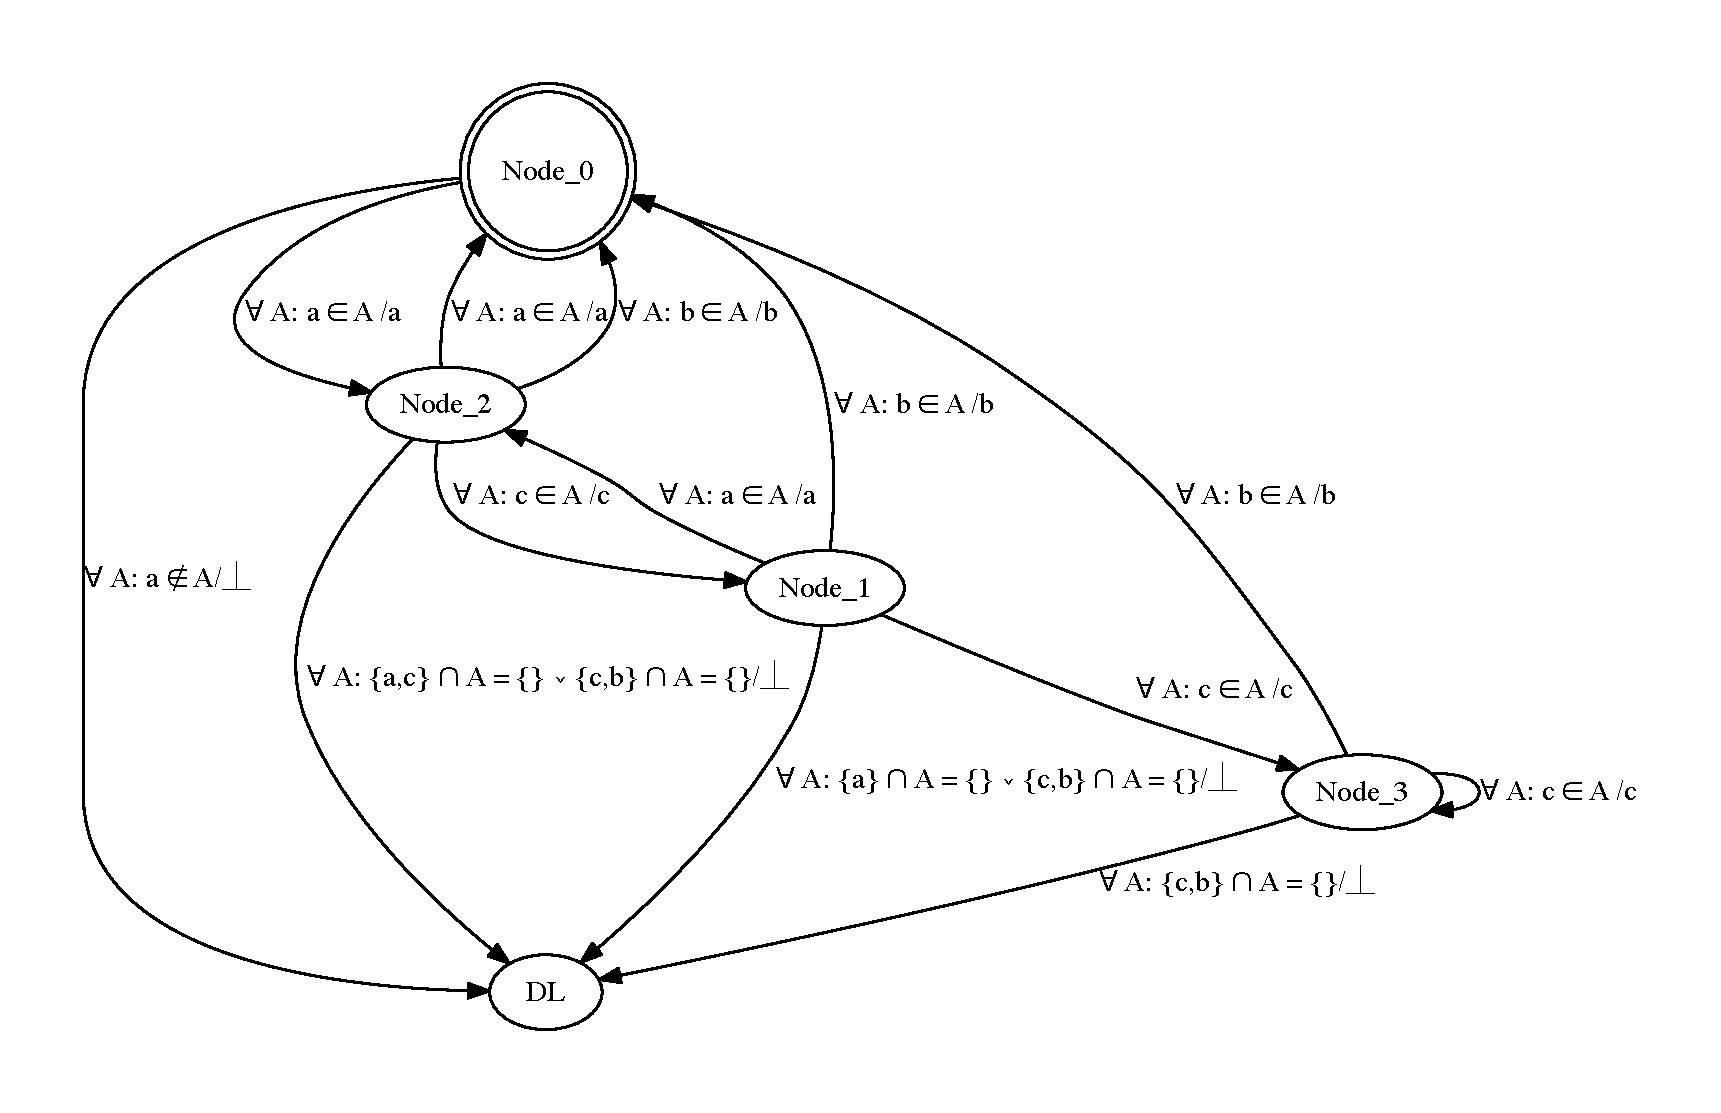
\includegraphics[width=\textwidth]{fsm0.pdf}
\end{center}
%%\vspace*{-10mm}
\caption{FSM resulting from applying the model map to CSP process $P$ from Example~\ref{ex:a}.}
 \label{fig:fsm0}
 \end{figure}
% ...................................................................................


\begin{example}{ex:b}
For the CSP process $P$ and its transition graph $G(P)$ discussed in
Example~\ref{ex:a}, the FSM $T(P)$ is depicted in Fig.~\ref{fig:fsm0}. For
displaying its transitions, we use notation
\[
(\text{condition}(A)) / e
\]
which stands for a set of transitions between the respective nodes: one transition per non-empty set $A\subseteq \Sigma$ fulfilling the specified condition.
The arrow
\[
\text{Node\_0} \xrightarrow{(a\in A) / a} \text{Node\_2},
\]
for example, stands for FSM transitions
\[
\begin{array}{l}
\text{Node\_0} \xrightarrow{\{a\}/a} \text{Node\_2} \\
\text{Node\_0} \xrightarrow{\{a,b\}/a} \text{Node\_2} \\
\text{Node\_0} \xrightarrow{\{a,c\}/a} \text{Node\_2} \\
\text{Node\_0} \xrightarrow{\{a,b,c\}/a} \text{Node\_2} \\
\end{array}
\]
\end{example}
%
\noindent%
We are now in the position to state and prove the theorem about the model map
fulfilling the satisfaction condition {\bf SC1} introduced in
Section~\ref{sec:transltt}. To this end, we first introduce five lemmas.

In the first lemma, we consider every trace $s$ of a process $P$ and the
state $n$ that it leads to in the normalised graph $G(P)$ of $P$. We show
that, for every transition from $n$ in the FSM, there are two possibilities.
The first is that the output $e$ is in the input $A$, so it is not $\bot$,
and, in this case, the trace $s.e$ is a trace of $P$, and the target state
$n'$ is that identified in $G(P)$. We use $s.e$ to denote the trace obtained
by adding the event $e$ to the end of $s$. The second possibility is that the
output is $\bot$, and in this case, we have a self-transition, that is, the
target state is $n$ itself, and $(s,A)$ is a failure of $P$.
%
\begin{lemma}\label{tran}
Let $s\in \trc(P)$ and $n=G(P)/s$ be the node of $G(P)$ corresponding to
process state $P/s$. Then for any $A \in \Sigma_I$, $e\in \Sigma_O\colon$
\begin{align*}
  (n,A,e,n')\in h\Leftrightarrow & (e\in A\wedge s.e\in \trc(P)\wedge n'=G(P)/s.e)\vee(e=\bot \wedge (s,A)\in \failure(P)\wedge n'=n)\end{align*}
\end{lemma}
\begin{proof}
  Let $s'=s.e\project \Sigma$.
  We consider the following two cases:
  \begin{itemize}
    \item[1.] Suppose $e=e$ for some $e\in \Sigma$. Then $s'=s.e$. By definition of $h$, we have
    \begin{align*}
      (n,A,e,n')\in h\Leftrightarrow & e\in A\wedge (n,e)\in {\text{\rm dom}}\, t\wedge n'=t(n,e)
      \\
      \Leftrightarrow& e\in A \wedge s.e\in \trc(P)\wedge n'=G(P)/s.e
    \end{align*}
    \item[2.] Suppose $e=\bot$. Then $s'=s$, and we can derive
    \begin{align*}
      (n,A,\bot,n')\in h\Leftrightarrow & A \in {\text {\rm Ref}}(P/s)\wedge n'=n
      \\
      \Leftrightarrow & (s,A) \in \failure(P)\wedge n'=n
    \end{align*}
  \end{itemize}
\end{proof}
%
%-----------------------------------------------------------------------------
%
Next, we use Lemma~\ref{tran} to relate traces and after states
of the process and the machine of arbitrary length.
%
\begin{lemma}\label{trac}
  Let $x/s \in (\Sigma_I\times\Sigma_O)^*$ and $s' = s\project \Sigma$.
  Then
  \[
    x/s \in L(T(P))\Rightarrow s' \in \trc(P) \wedge \underline q \after x/s = G(P)/s'.\]
\end{lemma}
\begin{proof}
  We prove the lemma by induction on $\#(x/y)$, the length of $x/y$.

  For the base case, suppose that $x/s = \varepsilon$, then $s = s' = \varepsilon$,
  which is a trace of every process, and $\underline q\after x/s = \underline
  n = G(P)/{\varepsilon }$. We recall that $\underline n$ is the initial node.

%  For the induction hypothesis, suppose the
%  statement holds for all $x/y\in (\Sigma_I\times\Sigma_O)^*$ with
%  $\#(x/y)=k$, for some $k\ge 0$. Let $x/y\in (\Sigma_I\times\Sigma_O)^*$
%  with $\#(x/y)=k$ and $x'/y'\in \Sigma_I\times \Sigma_O$. To perform the
%  induction step, let $y\project \Sigma=s$ and $y.y'\project \Sigma=s'$. Then
%  by the induction hypothesis we have $s\in\trc(P)$ and $\underline q\after
%  x/y=G(P)/s$. Since $x.x'/y.y'\in L(T(P))$, there is a transition
%  $(G(P)/s,x',y',n)\in h$ and $n=\underline q\after x.x'/y.y'$. By
%  Lemma~\ref{tran}, we have $s'\project\Sigma=(s.y')\project\Sigma\in
%  \trc(P)\wedge \underline q\after x.x'/y.y'=G(P)/s'$ for both cases
%  $y'\in\Sigma$ and $y'=\bot$.

  For the induction hypothesis, suppose the statement holds for all $x/s \in
  (\Sigma_I\times\Sigma_O)^*$ with $\#(x/s)=k$, for some $k\ge 0$. Let
  $x/s\in (\Sigma_I\times\Sigma_O)^*$ with $\#(x/s)=k$ and $A/e\in
  \Sigma_I\times \Sigma_O$. To perform the induction step, let $s\project
  \Sigma=s'$ and $(s.e) \project \Sigma=s''$. We need to prove that $s'' \in
  \trc(P)$ and $q\after x.A/s.e = G(P)/s''$. By the induction hypothesis, we
  have $s'\in\trc(P)$ and $\underline q\after x/s=G(P)/s'$. Since $x.A/s.e\in
  L(T(P))$, there is a transition $(G(P)/s',A,e,n)\in h$ with $n=\underline
  q\after x.A/s.e$. We consider two cases. In
  the first, $e \in A$, and so $e \in \Sigma$. We obtain the required results
  as follows. We note that
  %
  \begin{argue}
    s'' = (s.e) \project \Sigma = (s \project \Sigma).e = s'.e
  \end{argue}
  and $s'.e \in \trc(P)$ follows from Lemma~\ref{tran}. For $\underline q\after
  x.A/s.e$, we note that it is $n$, which, by Lemma~\ref{tran} is $G(P)/s'.e
  = G(P)/s''$ as shown above. In the second case, $e = \bot$. So, we note
  %
  \begin{argue}
    s'' = (s.\bot) \project \Sigma = s \project \Sigma = s'
  \end{argue}
  Lemma~\ref{tran} gives that $(s',A) \in \failure(P)$ and so $s' \in
  \trc(P)$. Finally, for $\underline q\after x.A/s.e$, we note that it is $n$, which, by
  Lemma~\ref{tran} is $G(P)/s' = G(P)/s''$ as shown above.
\end{proof}
%
%------------------------------------------------------------------
%
With the above two lemmas, we below relate the language of the FSM with the
trace and failure semantics of the CSP process that originated the FSM.
%
\begin{lemma}\label{exte}
Let $x/s\in L(T(P))$. Let $A/e\in \Sigma_I\times \Sigma_O$. Then
\begin{eqnarray*}
x.A/s.e\in L(T(P)) & \Leftrightarrow  &
\big(e\in A\wedge (s.e)\project \Sigma\in \trc(P)\big)\vee \big(e=\bot\wedge (s\project \Sigma, A)\in \failure(P)\big).
\end{eqnarray*}
\end{lemma}
\begin{proof}
Let $x/s\in L(T(P))$, and $A/e\in \Sigma_I\times \Sigma_O$. Then by
Lemma~\ref{trac}, we have $s'=s\project \Sigma\in \trc(P)$ and
$G(P)/s'=\underline q\after x/s$. From Lemma~\ref{tran} we have the following:
\[\begin{array}{lll}
&&x.A/s.e\in L(T(P)) \\&\Leftrightarrow & \exists n'\in Q: (G(P)/s,A,e,n')\in h\\
&\Leftrightarrow & (e\in A\wedge s.e\in \trc(P))\vee (e=\bot\wedge (s, A)\in \failure(P)\big)\\
&\Leftrightarrow & (e\in A\wedge (s.e)\project \Sigma\in \trc(P)\big)\vee \big(e=\bot\wedge (s\project \Sigma, A)\in \failure(P)\big)\end{array}
\]
\end{proof}
%
%----------------------------------------------------------------------------
%
Next we show that every trace of a process is represented in the FSM defined
by our map.
%
\begin{lemma}\label{cont}
For any $s\in \Sigma^*$,
\[s\in \trc(P) \Leftrightarrow \exists x\in \Sigma_I^*: x/s \in L(T(P)).\]
\end{lemma}
\begin{proof}
Let $s\in \Sigma^*$. We prove the lemma by induction on $\#s$. Suppose
$s=\varepsilon $, then $s\in \trc(P)$ because the empty trace is a trace of
every process.  Also, we recall that $(q,\varepsilon,\varepsilon,q) \in h$
for every $q$, by convention. So, $\varepsilon/\varepsilon \in L(T(P))$.
Therefore, $\exists x\in \Sigma_I^*: x/\varepsilon \in L(T(P))$ as required
for the base case.

For the induction step, suppose the statement holds for all $s\in \Sigma^*$
with $\#s=k$, for some $k\ge 0$. Let $s\in \Sigma^*$ with $\#s=k$ and
$e\in\Sigma$. Then we prove the equivalence by considering implication in each direction.
\begin{argue}
  s.e\in \trc(P)
  \\
  \Leftrightarrow s\in \trc(P)\wedge s.e\in \trc(P) & prefix closure of CSP traces
  \\
  \Leftrightarrow \exists x\in \Sigma_I^*: x/s\in L(T(P))\wedge s.e\in \trc(P) & induction hypothesis
  \\
  \Rightarrow \exists x\in \Sigma_I^*: x.\{e\}/s.e\in L(T(P))& {\text{Lemma~\ref{exte}}} and $(s.e) \project \Sigma = s.e$
  \\
  \Rightarrow \exists x\in \Sigma_I^*: x/s.e\in L(T(P)) & predicate calculus
\end{argue}
For the implication in the other direction, we have the following.
\begin{argue}
  \exists x\in \Sigma_I^*: x/s.e \in L(T(P))
  \\
  \Leftrightarrow \exists x\in \Sigma_I^*\wedge \exists x'\in \Sigma_I: x/s\in L(T(P))\wedge x.x'/s.e\in L(T(P))
  & in $x/s.e$, we have $\# x = \# s.e$
  \\
  \Rightarrow s.e\in \trc(P)& {\text{Lemma~\ref{trac}}} and $(s.e) \project \Sigma = s.e$
\end{argue}
\end{proof}
%
%----------------------------------------------------------------------------
%
Similarly, every failure of a process is represented in the FSM defined
by our map.
\begin{lemma}\label{conf}
For any $s\in \Sigma^*$ and $R\in \Sigma_I$,
\[(s,R)\in \failure(P)\Leftrightarrow \exists x\in \Sigma_I^*: x.R/s.\bot \in L(T(P))\]
\end{lemma}
\begin{proof}
\begin{argue}
  \exists x\in \Sigma_I^*: x.R/s.\bot\in L(T(P))
  \\
  \Leftrightarrow \exists x\in \Sigma_I^*: x/s\in L(T(P))\wedge x.R/s.\bot\in L(T(P))
  & definition of $L$
  \\ %
  \Leftrightarrow (s,R)\in \failure(P)& {\text {Lemma~\ref{exte} and Lemma~\ref{cont}}}
\end{argue}
\end{proof}
%
%------------------------------------------------------------------------------
%
We finally get to the main result of this section, which establishes that our
map satisfies {\bf SC1}. The conformance relations are failures refinement
and FSM reduction.
\begin{theorem}
Let $P,Q$ be two CSP processes over the same alphabet $\Sigma$. Then
$T(Q)\preceq T(P) \Leftrightarrow P\,\sqsubseteq_F\, Q$.
\end{theorem}
\begin{proof}
First, suppose $T(Q)\preceq  T(P)$. Let $s\in \Sigma^*, A\in \Sigma_I$.
\[
  \begin{array}{llll}
    s\in \trc(Q) & \Leftrightarrow & \exists x\in \Sigma_I^*: x/s\in L(T(Q)) & [{\text {Lemma~\ref{cont}}}]
    \\
    & \Rightarrow & \exists x\in \Sigma_I^*: x/s\in  L(T(P)) & [T(Q)\preceq T(P)]
    \\
    &\Leftrightarrow & s \in \trc(P) & [{\text {Lemma~\ref{cont}}}]
  \end{array}
\]
%
\[
  \begin{array}{llll}
    (s,A)\in \failure(Q) & \Leftrightarrow & \exists x\in \Sigma_I^*: x.A/s.\bot \in L(T(Q)) & [{\text {Lemma~\ref{conf}}}]
    \\
    & \Rightarrow & \exists x\in \Sigma_I^*: x.A/s.\bot \in L(T(P)) & [T(Q)\preceq T(P)]
    \\
    & \Leftrightarrow & (s,A)\in \failure(P) & [{\text {Lemma~\ref{cont}}}]
  \end{array}
\]
%
Hence $T(Q)\preceq  T(P)\Rightarrow P\,\sqsubseteq_F\, Q$.

For the implication in the other direction, now suppose $P\,\sqsubseteq_F\,
Q$. We prove by induction on $\#(x/s)$ that for any $x/s\in (\Sigma_I\times
\Sigma_O)^*$,  $x/s\in L(T(Q))\Rightarrow x/s\in L(T(P))$ holds. It is
trivial if $\#(x/s)=0$ because $x = s = \varepsilon$, which is in the
language of every FSM. Suppose $x/s\in L(T(Q))\Rightarrow x/s\in L(T(P))$
holds for any $x/s\in (\Sigma_I\times \Sigma_O)^*$ of length $k\ge 0$. For
any $x/s\in (\Sigma_I\times \Sigma_O)^*$ of length $k$ and for any $A/e\in
\Sigma_I\times \Sigma_O$. Let $s' = s\project \Sigma$ and $s'' = (s.e)\project
\Sigma$.
%
\begin{argue}
  x.A/s.e\in L(T(Q))
  \\
  \Rightarrow x/s\in L(T(Q))\wedge \big((e\in A\wedge s'\in \trc(Q))\vee (e=\bot\wedge (s',A)\in \failure(Q))\big)
  \\
  & prefix closure of $L(T(Q))$ and Lemma~\ref{exte}
  \\
  \Rightarrow x/s\in L(T(P))\wedge \big((e\in A\wedge s'\in \trc(P)\big)\vee (e=\bot\wedge (s',A)\in \failure(P))\big)
  \\
  & induction hypothesis and $ P\,\sqsubseteq_F\, Q$
  \\
  \Rightarrow x.A/s.e\in L(T(P)) & Lemma~\ref{exte}
\end{argue}
%
Hence $ P\,\sqsubseteq_F\, Q \Rightarrow T(Q)\preceq  T(P)$.
\end{proof}
%
In the next section, we consider {\bf SC2} for the test case map.



% ==========================================================================
\subsection{A Test Case Map from Finite State Machines to CSP Processes}
\label{sec:tcmap}
% ==========================================================================

In this section, we first of all define a notion of test cases for FSM and
then for CSP. Afterwards, we define a map between these test cases that satisfies
{\bf SC2} as required.

% -------------------------------------------------------------------------
\subsubsection{FSM Test Cases}

Following~\cite{DBLP:conf/hase/PetrenkoY14},
an \emph{adaptive FSM test case}
\[
tc_\text{FSM}=(Q,\ii q,\Sigma_I,\Sigma_O,h,in)
\]
is a nondeterministic, observable, output-complete, acyclic FSM that provides
only a single input in any given state. Running in intersection mode with the
SUT, the test case provides a specific input to the SUT determined by the
current state of the test case. It accepts every output and transits either
to a fail-state FAIL, if the output is wrong according to the test
objectives, or to the next test state uniquely determined  by the processed
input/output pair. Another state PASS indicates that the test has been
completed without failure. Both FAIL and PASS are deadlock states.

Since the test case state determines the input for all of its outgoing transitions, this input is typically used as a state label, and the outgoing transitions are just labelled by the possible outputs. A function $in : Q -\{  \text{PASS}, \text{FAIL} \}
\fun\Sigma_I$ maps the states to these inputs. Termination states
of the FSM are not labelled with further inputs.

There is no requirement that an FSM test case running in intersection mode against
an FSM $M$ acting as SUT should {\it always} reach the PASS state. Since the SUT may be nondeterministic, it may perform a joint test execution that blocks before
the test case's PASS state is reached. In such a case, the result of the test execution is \emph{inconclusive}. Due to nondeterminism, for $M$ to pass a test case, it
has to be 
checked that {\it every possible} test execution of  $tc_\text{FSM}$ against $M$
terminates either in PASS, or that the result remains inconclusive. If one execution ends in FAIL, the test verdict is FAIL. More formally,
\[
M\ \passred\ tc_\text{FSM} \equiv
\big(
\forall x/y \in L(M)\cap L(tc_\text{FSM}): \ii q\after(x/y) \neq FAIL
\big).
\]
It will turn out in the exposition below that this pass criterion is appropriate for 
testing the reduction conformance relation. For equivalence testing, it is also of 
interest whether {\it all} pass-traces of an adaptive test case are contained
in the language of the FSM under test. This induces a second pass criterion specified by
\begin{eqnarray*}
M\ \passeq\ tc_\text{FSM} & \equiv &
\big(
\forall x/y \in L(M)\cap L(tc_\text{FSM}): \ii q\after(x/y) \neq \text{FAIL}
\big) \wedge
\\ & &
\big(
\forall x/y \in L(tc_\text{FSM}): \ii q\after(x/y) = \text{PASS} \Rightarrow
x/y\in L(M)
\big)
\end{eqnarray*}

\begin{example}{ex:xx}
Consider the FSM test case depicted in Fig.~\ref{fig:fsm0tc} which is specified
for the same input and output alphabets as defined for  the FSM presented in Example~\ref{ex:b}. The test case is passed by the FSM from Example~\ref{ex:b}, because
intersecting the two state machines results in an FSM which always reaches the PASS state.
\end{example}

While adaptive test cases are an operational representation of tests, an alternative, equivalent, denotational description can be given by means of \emph{pass-traces} and \emph{fail-traces}, as introduced in~\cite{huang_peleska_2017sttt}: a test case 
$U = (\xpass U,\xfail U)$ consists of two sets of traces 
$\xpass U, \xfail U\subseteq L(M)$, such that $\xpass U \cap \xfail U = \varnothing$.





We introduce two pass-criteria that will be used later on to distinguish tests for equivalence and tests for refinement.
\begin{eqnarray}
M\ \passeq\ U & \equiv & \xpass U \subseteq L(M) \wedge L(M)\cap \xfail U =\varnothing
\label{eq:passeq}
\\
M\ \passred\ U & \equiv & L(M)\cap \xfail U =\varnothing
\label{eq:passred}
\end{eqnarray}
By definition, both pass criteria require that none of the fail-traces are contained
in the language of the FSM under test. This suffices when testing for language inclusion,
as defined in the pass-criterion (\ref{eq:passeq}).
When testing for language equivalence as specified in (\ref{eq:passeq}), it is additionally required that {\it all} pass traces need to be contained in $L(M)$.


It is easy to see how adaptive test cases can be transformed into their denotational representation. Conversely, it is easy to transform a test case $U = (\xpass U,\xfail U)$
into one or more adaptive test cases. Since the denotational test case representation
is very general, however, it is not guaranteed that they can always be transformed into {\it a single} adaptive test case: this is due to the fact that adaptive test cases
are required to be single-input.
\begin{example}{ex:tctransform}
Consider again the adaptive FSM test case depicted in Fig.~\ref{fig:fsm0tc}.
Its pass-traces and fail-traces are given by
\begin{eqnarray*}
\xpass U & =  & \{ (\{a,b,c\}/a).(\{c\}/c).(\{c\}/\bot).(\{a\}/a),
\\ & & \ \ (\{a,b,c\}/a).(\{c\}/c).(\{c\}/c).(\{c\}/c)
\}
\\ & & {~} \\
\xfail U & = & \{ (\{a,b,c\}/b), (\{a,b,c\}/c), (\{a,b,c\}/\bot),
\\ & & \ \ (\{a,b,c\}/a).(\{c\}/a), (\{a,b,c\}/a).(\{c\}/b), (\{a,b,c\}/a).(\{c\}/\bot),
\\ & & \ \ (\{a,b,c\}/a).(\{c\}/c).(\{c\}/a), (\{a,b,c\}/a).(\{c\}/c).(\{c\}/b),
\\ & & \ \ (\{a,b,c\}/a).(\{c\}/c).(\{c\}/\bot).(\{a\}/b),
(\{a,b,c\}/a).(\{c\}/c).(\{c\}/\bot).(\{a\}/c),
\\ & & \ \ 
(\{a,b,c\}/a).(\{c\}/c).(\{c\}/\bot).(\{a\}/\bot),
\\ & & \ \ (\{a,b,c\}/a).(\{c\}/c).(\{c\}/c).(\{c\}/a),
(\{a,b,c\}/a).(\{c\}/c).(\{c\}/c).(\{c\}/b),
\\ & & \ \ 
(\{a,b,c\}/a).(\{c\}/c).(\{c\}/c).(\{c\}/\bot)
\}
\end{eqnarray*}
This can be directly derived by performing a reachability analysis for the states PASS and FAIL, respectively, using the graph representation in Fig.~\ref{fig:fsm0tc}.
\end{example}



% ...................................................................................
 \begin{figure}
 %%\hspace*{-40mm}
 \begin{center}
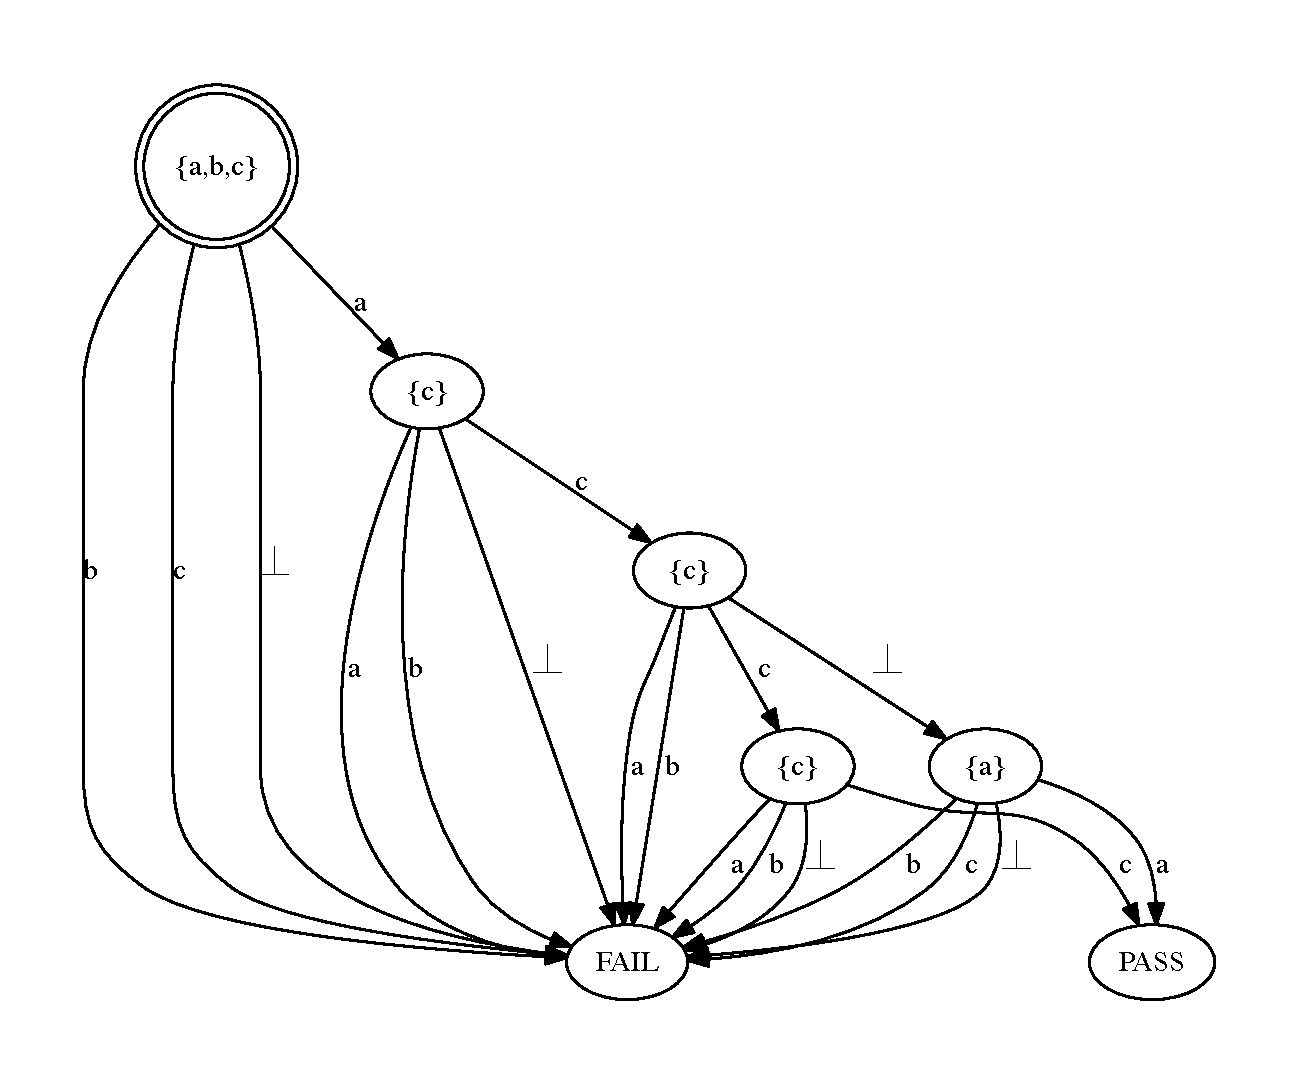
\includegraphics[width=.8\textwidth]{fsm0tc.pdf}
\end{center}
%%\vspace*{-10mm}
\caption{An FSM test case which is passed by the FSM presented in Example~\ref{ex:b}.}
 \label{fig:fsm0tc}
 \end{figure}
% ...................................................................................


% =========================================================================
\subsubsection{FSMs in the Range of the Model Map}
\label{sec:fsmT}
% =========================================================================

We will now state some facts about FSMs in the range of the model map; these will be exploited in the definition of effective CSP test cases for failures equivalence and
failures refinement. They are also needed in the proof of the satisfaction condition
{\bf SC2} showing the correctness of the test case map to be constructed below.


\begin{lemma}\label{lemma:fsmT}
Let $M = (Q,\ii q, \Sigma_I,\Sigma_O,h)$ be an FSM in the range of the model map $T$. 
Then the following facts hold for all $q\in Q$, $A, A_i\in\Sigma_I$, $e\in\Sigma$, and 
$u_i \in (\Sigma_I\times\Sigma_O)^*$.
\begin{eqnarray}
(A_1/\bot).(A_2/\bot)\in L(q) & \Leftrightarrow  &(A_2/\bot).(A_1/\bot)\in L(q)
\label{eq:eq1}
\\
u_1.(A/\bot).u_2\in L(q) & \Leftrightarrow & u_1.u_2\in L(q) \wedge 
(A/\bot)\in L(\ii q\after u_1)
\label{eq:eq2}
\\
(A_1/\bot) \in L(q) \wedge A_2\subseteq A_1 & \Rightarrow & (A_2/\bot) \in L(q)
\label{eq:eq3}
\\
(A_1/e) \in L(q) \wedge A_1\subseteq A_2 & \Rightarrow & (A_2/e) \in L(q)
\label{eq:eq4}
\\
(A/e) \in L(q) & \Rightarrow & e\in A
\label{eq:eq5}
\\
(A_1/e) \in L(q) \wedge (A_2/e) \in L(q) & \Rightarrow & q\after(A_1/e) = q\after (A_2/e)
\label{eq:eq6} 
\end{eqnarray}
\end{lemma}
\begin{proof}
Formulas (\ref{eq:eq1}) and (\ref{eq:eq2}) are  direct consequences of the fact that all
transitions labelled with output $\bot$ are self-loops. Formula (\ref{eq:eq3})  is 
a direct consequences of the fact that refusals are subset-closed, and  
$(A_1/\bot) \in L(q)$ if and only if $A_1$ is contained in some refusal of the
CSP transition graph node $q$ (recall that the model map maps graph nodes to FSM states
in one-one fashion). 
For proving Formula (\ref{eq:eq4}), we note that $(A_1/e) \in L(q)$ if and only if
the CSP transition graph contains an outgoing transition from graph node $q$ which is labelled by $e$. Since $A_2$ is supposed to be a super-set of $A_1$, this property holds for $A_2$ as well. Formula (\ref{eq:eq5}) follows from the definition of the 
model map $T$ which specifies $e\in A$ as a necessary condition for FSM transitions $h(q,A,e,q')$ with $e\in \Sigma$.
Formula (\ref{eq:eq6}) follows from the fact that by definition of the model map, 
$h(q,A_1,e,q')$ requires $t(q,e) = q'$ and $h(q,A_2,e,q'')$ requires $t(q,e) = q''$, where $t$ is the transition function of the normalised CSP transition graph. Since $t$ is a function, $q'=q''$ follows.
\end{proof}

The following theorem states that complete test suites for FSMs in the range of the 
model map can be simplified in such a way, that every pass-trace contains at most one
self-transition $(A/\bot)$, and this only occurs at the end of the trace.

\begin{theorem}\label{th:fsmT}
Let $M = (Q,\ii q, \Sigma_I,\Sigma_O,h)$ be an FSM in the range of the model map $T$. 
Let $\TS$ be  a complete test suite for verifying reduction or refinement with a fault domain that is also in the range of the model map. Let $\TS'$ be another test suite satisfying the following conditions.
\[
\def\arraystretch{1.2}
\begin{array}{l}
\text{[Condition~1.]}
\\
  \forall U = (\xpass U,\xfail U)\in\TS: \exists  U' = (\xpass U',\xfail U')\in\TS':
\\\tabc
\big( \forall u\in \xpass U: \exists u'\in \xpass U': 
 last(u) = last(u') \wedge front(u\project(\Sigma_I\times\Sigma)) = front(u')\big)
 \wedge {} 
 \\\tabc
 \big( \forall u\in \xfail U: \exists u'\in \xfail U': 
 last(u) = last(u') \wedge front(u\project(\Sigma_I\times\Sigma)) = front(u')\big)
 \\ {~}
 \\
 \text{[Condition~2.]}
\\
  \forall U = (\xpass U,\xfail U)\in\TS, A\in\Sigma_I: 
  \exists  U' = (\xpass U',\xfail U')\in\TS':
\\\tabc
\big( \forall u.(A/\bot).v\in \xpass U: \exists u'\in \xpass U': 
 u' = (u\project(\Sigma_I\times\Sigma)).(A/\bot)
 \big)
 \wedge {} 
 \\\tabc
\big( \forall u.(A/\bot).v\in \xfail U: v \neq\varepsilon\Rightarrow\exists u'\in \xpass U': 
 u' = (u\project(\Sigma_I\times\Sigma)).(A/\bot)
 \big)
\end{array}
\def\arraystretch{1}
\]
Then $\TS'$ is also complete for the same conformance relation and fault domain.
\end{theorem}
\begin{proof}
We first consider the pass-criterion $\passeq$ for language equivalence.
It first has to be shown that $\TS'$ is also sound; this means that conforming 
implementations will pass all test cases of $\TS'$. Suppose therefore that
$M' \sim M$ for  $M' = (Q',\ii q', \Sigma_I,\Sigma_O,h')$ and let $U' = (\xpass U',\xfail U')\in \TS'$. Let $u'\in\xpass U'$. We have to show that $u'\in L(\ii q)$. From Condition~1 and Condition~2 we conclude that
there exists a test case $U = (\xpass U,\xfail U)\in \TS$ and a pass-trace
$u\in\xpass U$ such that (1) 
$last(u) = last(u') \wedge front(u\project(\Sigma_I\times\Sigma)) = front(u')$ 
or (2) $u = w.(A/\bot).v$ and $u' = w\project(\Sigma_I\times\Sigma).(A/\bot)$.
Since $\TS$ is sound, we know that $u\in L(\ii q')$.


In Case (1), Lemma~\ref{lemma:fsmT}, (\ref{eq:eq2}) implies that $u'\in L(\ii q')$,
because $u'$ has been constructed from $u$ by deleting  I/O-pairs $(A/\bot)$.
In Case (2), $u' = w\project(\Sigma_I\times\Sigma).(A/\bot)$ for some
$u = w.(A/\bot).v\in\xpass U$. Since $w.(A/\bot).v\in L(\ii q')$, prefix closure of languages gives us $w.(A/\bot)\in L(\ii q')$. 
Again,  Lemma~\ref{lemma:fsmT}, (\ref{eq:eq2}) implies that $u'\in L(\ii q')$. 

Now it has to be shown that no fail-trace $a' \in \xfail U'$ is contained in the language of $M'$. To this end, we observe that  $a'$ is the prefix of some fail-trace $a\in\xfail U$, where some $(A/\bot)$ I/O-events have been deleted. 
Lemma~\ref{lemma:fsmT}, (\ref{eq:eq2}) implies that 
$a'\in L(M') \Leftrightarrow a \in L(M')$. Since $\TS$ is sound and $M'$ conforms to $M$, $a$ is not an element of $L(M')$. Therefore, $a'\not\in L(M')$, so $M'$ also passes the test $U'$.
This
completes the proof that $\TS'$ is sound for showing language equivalence.

To show that $\TS'$ is exhaustive for language equivalence, suppose that $M'\not\sim M$.
Since $\TS$ is complete by assumption, this implies  the existence of a 
test case $U = (\xpass U,\xfail U)\in\TS$ and (1) a fail-trace $a\in\xfail U$ such that
$u\in\L(\ii q')$, or (2) the existence of a pass-trace $u\in\xpass U$ which is {\it not} contained in $L(\ii q')$.

For Case (1), Condition~1 ensures the existence of a fail-trace $a'$ which is derived 
from $a$ by deleting some $(A/\bot)$ I/O-pairs. From Lemma~\ref{lemma:fsmT}, (\ref{eq:eq2}), we know that $a'$ is also in the language of $M'$. Therefore, $M'$ 
also fails the $\TS'$-test case containing fail-trace $a'$. For Case (2), 
Condition~1 yields the existence of as pass-trace $u'$ in some test case of $\TS'$
which is constructed from $u$ by deleting some $(A/\bot)$ I/O-pairs. Now
Lemma~\ref{lemma:fsmT}, (\ref{eq:eq2}) implies that $u'\not\in L(\ii q')$ because
$u\not\in L(\ii q')$. Therefore, the $\TS'$ test case containing $u'$ also fails for $M'$. 
 

Next, we consider the pass criterion $\passred$ for reduction. First, the soundness of
$\TS'$ is shown. To this end, we only have to prove that the fail-traces of $U'$ are not contained in $L(M')$ if $M'$ is a reduction of $M$. This follows from the same argument as applied above for the language equivalence case. To prove exhaustiveness, 
assume that $a\in L(M')$ for some fail-trace of a test case of $\TS$. Now we can
apply the same argument as for the exhaustiveness Case (1) described for equivalence testing above to prove the existence of a fail-trace $a'$ from test suite $\TS'$ which is also contained in $M'$'s language. This completes the proof. 
\end{proof}

Next, it is shown that every test case in denotational representation can be
transformed into a set of adaptive test cases.

\begin{theorem}
Let $U = (\xpass U, \xfail U)$ be a test case. Then there exists a set ${\cal A}(U)$
of adaptive test cases that are equivalent to $U$ in the sense that 
\begin{eqnarray*}
M\ \passeq\ U & \Leftrightarrow & \forall U_A\in {\cal A}(U): M\ \passeq\ U_A
\\
M\ \passred\ U & \Leftrightarrow & \forall U_A\in {\cal A}(U): M\ \passred\ U_A
\end{eqnarray*}
\end{theorem}
\begin{proof}
aa
\end{proof}

\begin{algorithm}
\caption{Conversion of test case $U=(\xpass U,\xfail U)$ to set of adaptive test cases.}
\label{algo:a1}
\SetKwFunction{createFromPassTrace}{createFromPassTrace}
\SetKwFunction{createFromFailTrace}{createFromFailTrace}
\SetKwFunction{extendByPassTrace}{extendByPassTrace}
\SetKwFunction{extendByFailTrace}{extendByFailTrace}
\SetKwFunction{makeComplete}{makeComplete}

\KwData{Finite test case $U=(\xpass U,\xfail U)$.}
\KwResult{Finite set of adaptive test cases equivalent to $U$.}
\Begin{
${\cal A}(U) := \varnothing$\;
$P := \xpass U$ \;
$F := \xfail U$ \;
 \While{$P\cup F\neq\varnothing$} {
   \If {$P \neq \varnothing$} {
      $tc = \createFromPassTrace{P}$\;
      \lWhile{$\extendByPassTrace{$tc,P$}$}{}
      \lWhile{$\extendByFailTrace{$tc,P$}$}{}
      \makeComplete{$tc$}\;
      ${\cal A}(U) := {\cal A}(U)\cup \{ tc \}$\;
   }
   \Else {
    $tc := \createFromFailTrace{P}$\;
      \lWhile{$\extendByFailTrace{$tc,P$}$}{}
      \makeComplete{$tc$}\;
      ${\cal A}(U) := {\cal A}(U)\cup \{ tc \}$\;
   } 
 }
 \Return{${\cal A}(U)$}\;
}
\end{algorithm}


\begin{algorithm}
\caption{Initialisation of an adaptive test case with pass-trace.}
\label{algo:aInitP}
\SetKwFunction{createFromPassTrace}{TestCase createFromPassTrace}
\SetKwFunction{createTestCase}{createTestCase}
\createFromPassTrace{{\bf inout} $P : \power((\Sigma_I\times \Sigma_O)^*)$}
{
\Begin{
Select trace $\pi$ from $P$\;
$P := P - \{ \pi\}$\;
\Return{\createTestCase{$\pi,\text{PASS}$}}\;
}
}
\end{algorithm}


\begin{algorithm}
\caption{Initialisation of an adaptive test case with fail-trace.}
\label{algo:aInitF}
\SetKwFunction{createFromFailTrace}{TestCase createFromFailTrace}
\SetKwFunction{createTestCase}{createTestCase}
\createFromFailTrace{{\bf inout} $F : \power((\Sigma_I\times \Sigma_O)^*)$}
{
\Begin{
Select trace $\pi$ from $F$\;
$F := F - \{ \pi\}$\;
\Return{\createTestCase{$\pi,\text{FAIL}$}}\;
}
}
\end{algorithm}

\begin{algorithm}
\caption{Initialisation of an adaptive test case with given trace and end-state.}
\label{algo:aInit}
\SetKwFunction{createTestCase}{TestCase createTestCase}
\createTestCase{{\bf in} $\pi : (\Sigma_I\times \Sigma_O)^*$, {\bf in} endState : State}
{
\Begin{
{\bf let}\ $\pi = (x_0\dots x_{\#\pi-1})/(y_0\dots y_{\#\pi-1})$\;
$Q := \{ \ii q, q_1, \dots, q_{\#\pi-1}, endState \}$\;
$tc := (Q,\ii q, \Sigma_I,\Sigma_O,h,in)$\;
$in := \{ \ii q \mapsto x_0, q_1\mapsto x_1,\dots,q_{\#\pi-1}\mapsto x_{\#\pi-1}  \}$\;
$h := \{ (\ii q,x_0,y_0,q_1)  \} \cup \{ (q_i,x_i, y_i,q_{i+1})~|~i= 1,\dots\#\pi - 2  \}
\cup \{ (q_{\#\pi-1}, x_{\#\pi-1}, y_{\#\pi-1},endState) \}$\;
\Return{$(Q,\ii q,\Sigma_I,\Sigma_O,h,in)$}\;
}
}
\end{algorithm}


\begin{algorithm}
\caption{Extend adaptive test case under construction with pass-trace.}
\label{algo:aExtendP}
\SetKwFunction{extendByPassTrace}{$\mathbb{B}$ extendByPassTrace}
\SetKwFunction{extendByTrace}{extendByTrace}
\extendByPassTrace{{\bf inout} tc : TestCase, {\bf inout}\ $P : \power((\Sigma_I\times \Sigma_O)^*)$ }
{
\Begin{
\For{$\pi\in P$} {
\If {\extendByTrace{$tc,\pi,\mbox{\rm PASS}$}} {
$P := P - \{ \pi\}$\;
\Return{$\ist$}\;
}
}
\Return{$\isf$}\;
}
}
\end{algorithm}


\begin{algorithm}
\caption{Extend adaptive test case under construction with fail-trace.}
\label{algo:aExtendF}
\SetKwFunction{extendByFailTrace}{$\mathbb{B}$ extendByFailTrace}
\SetKwFunction{extendByTrace}{extendByTrace}
\extendByFailTrace{{\bf inout} tc : TestCase, {\bf inout}\ $F : \power((\Sigma_I\times \Sigma_O)^*)$ }
{
\Begin{
\For{$\pi\in F$} {
\If {\extendByTrace{$tc,\pi,\mbox{\rm FAIL}$}} {
$F := F - \{ \pi\}$\;
\Return{$\ist$}\;
}
}
\Return{$\isf$}\;
}
}
\end{algorithm}



\begin{algorithm}
\caption{Try to extend test case by given trace and end-state.}
\label{algo:aExtend}
\SetKwFunction{extendByTrace}{$\mathbb{B}$ extendByTrace}
\extendByTrace{{\bf inout} tc : TestCase, {\bf in}\ $\pi : (\Sigma_I\times \Sigma_O)^*$, {\bf in} endState : State}
{
\Begin{
{\bf let}\ $\pi = \pi_1.\pi_2 \wedge \pi_1\in L(tc) \wedge \pi_1.\pi_2(0)\not\in L(tc)
\wedge \pi_2 = (x_0\dots x_m)/(y_0\dots y_m)$ \;
{\bf let}\ $tc = (Q,\ii q,\Sigma_I,\Sigma_O,h,in) \wedge n = |Q|$\;
$q := \ii q\after \pi_1$\;
\lIf{$in(q) \neq x_0 $} {\Return{$\isf$}}
$Q := Q\cup \{ q_{n+1},\dots,q_{n+m}, endState  \}$\;
$h := h\cup \{ (q,x_0,y_0,q_n) \} \cup
\{ (q_{n+j},x_j,y_j,q_{n+j+1})~|~j=1,\dots,m-1 \} \cup \{ (q_{n+m},x_m,y_m,endState) \}$\;
$in := in\cup \{ q_{n+j} \mapsto x_j~|~j=1,\dots,m \}$\;
\Return{$\ist$}\;
}
}
\end{algorithm}



\begin{algorithm}
\caption{Make test case output-complete.}
\label{algo:aComplete}
\SetKwFunction{makeComplete}{makeComplete}
\makeComplete{{\bf inout} tc : TestCase}
{
\Begin{
{\bf let}\ $tc = (Q,\ii q,\Sigma_I,\Sigma_O,h,in) \wedge n = |Q|$\;
\For{$q \in Q\setminus \{ \mbox{\rm PASS}, \mbox{\rm FAIL}, \mbox{\rm INC}\}$}{
\For{$y\in\Sigma_O$}{
  \lIf{$(in(q)/y)\not\in L(q)$}{
     $Q := Q\cup \{ \mbox{\rm INC} \}$\;
     $h := h\cup \{ (q,in(q),y,\mbox{\rm INC}) \}$
}
}
}
}
}
\end{algorithm}



% -------------------------------------------------------------------------
\subsubsection{CSP Test Cases}
\label{sec:csptc}
A \emph{CSP test case} $tc_\text{CSP}$  is a terminating process with alphabet
$\Sigma\cup\{\dag,\bot,\tick \}$, where the extra events stand for
(1) test  verdict FAIL ($\dag$), (2) timeout ($\bot$), and (3) test
 verdict PASS ($\tick$). The test case runs in parallel with the SUT $P$,
 synchronising over all events from the visible alphabet $\Sigma$ of $P$. This is
 expressed by the formula
 \[
 P\parallel[\Sigma] tc_\text{CSP}.
 \]

 In analogy to FSM test cases, a CSP process $P$ passes a test case $tc_\text{CSP}$
 if the traces of the parallel composition do not contain the failure event, that is,
 \[
 P\ \pass\ tc_\text{CSP} \equiv \big(
 \forall s\in\trc(P\parallel[\Sigma] tc_\text{CSP}): (s\project \{\dag\}) = \varepsilon
 \big)
 \]


 In principle, very general classes of CSP processes can be
 used for testing, as introduced, for example,
 in~\cite{DBLP:conf/fm/PeleskaS96,peleska1997a}. For the purpose of this paper, however, we can restrict the possible variants of CSP test cases to the ones that are in the range of the test case map which is constructed next.


% -------------------------------------------------------------------------
\subsubsection{Test Case Map}

The test case map $T^* :TC(FSM) \pfun TC(CSP)$ is specified with respect to a fixed
CSP process alphabet $\Sigma$ extended by the events $\{\dag,\bot,\tick \}$ introduced
above
and the associated FSM input and output alphabets
$\Sigma_I = \power(\Sigma)-\{\varnothing\}$ and $\Sigma_O=\Sigma\cup \{\bot \}$.
As a consequence of Theorem~\ref{th:fsmT}, the domain of $T^*$ may be restricted to
test cases $U = (\xpass U,\xfail U)$ of the form where every pass-trace $u\in\xfail U$
or fail-trace $a\in\xfail U$ contains I/O-pairs $(A/\bot), A\in \Sigma_I$, if any, at the very last element of the trace. Theorem~\ref{th:fsmT} implies that {\it any} complete
test suite for FSMs in the range of the model map $T$ can be represented by means of
test cases fulfilling this condition.





Given such an FSM test case $tc_\text{FSM}=(Q,\ii q,\Sigma_I,\Sigma_O,h,in)$,
the image $T^*(tc_\text{FSM})$ is the CSP process $tc_\text{CSP}$ specified
as follows.
\begin{eqnarray*}
tc_\text{CSP} & = & tc(\ii q)
\\
tc(q) & = & \big( e :  A(q) \then  tc(q\after (in(q)/e)) \big)
\\ & & \extchoice
 \big( e : A_\text{PASS}(q)   \then \tick \then \Skip \big)
\\ & & \extchoice
 \big( e : A_\text{FAIL}(q) \then \dag \then \Skip \big)
\\ & &
\\
A(q) & = & \{ a\in in(q)~|~q\after (in(q)/a)\notin \{\text{PASS},\text{FAIL}\} \}
\\
A_\text{PASS}(q) & = & \{ a\in in(q)\cup\{\bot\}~|~q\after(in(q)/a) = \text{PASS} \}
\\
A_\text{FAIL}(q) & = & \{ a\in in(q)\cup\{\bot\}~|~q\after(in(q)/a) = \text{FAIL} \}
\end{eqnarray*}


%\begin{eqnarray*}
%tc_\text{CSP} & = & tc(\ii q)
%\\
%tc(q) & = & \big( e :  A(q) \then  tc(q\after (in(q)/e)) \big)
%\\ & & \extchoice
% \big( e : A_\text{PASS}(q)   \then \tick \then \Skip \big)
%\\ & & \extchoice
% \big( e : A_\text{FAIL}(q) \then \dag \then \Skip \big)
%\\ & &
%\\
%A(q) & = & \{ a\in in(q)\cup\{\bot\}~|~q\after (in(q)/a)\notin \{\text{PASS},\text{FAIL}\} \}
%\\
%A_\text{PASS}(q) & = & \{ a\in in(q)\cup\{\bot\}~|~q\after(in(q)/a) = \text{PASS} \}
%\\
%A_\text{FAIL}(q) & = & \{ a\in in(q)\cup\{\bot\}~|~q\after(in(q)/a) = \text{FAIL} \}
%\end{eqnarray*}

@todo update text to new test case version.
Intuitively speaking, $tc_\text{CSP}$ offers in each test step the same events to
the CSP process to be tested as the FSM test case offers to the FSM under test.
These events are specified in each non-terminating test step by $in(q)$, where
$q$ is the current state of the FSM test case $tc_\text{FSM}$. While the FSM test
case offers these events a single set-valued member of the input alphabet $\Sigma_I$
to the FSM under test, the CSP test offers the same to the SUT by means of an external choice, so that it just depends on the SUT which event to choose. In addition to the
events from $in(q)$, the CSP test case
accepts the event $\bot$ which is not shared with
the SUT but represents a timeout event provided by the testing environment to indicate
that the SUT is blocked without accepting any of the events in $in(q)$.

The events offered/accepted by the CSP test in state $tc(q)$ are partitioned into
3 sets $A(q)$, $A_\text{PASS}(q)$, and $A_\text{FAIL}(q)$. The disjointness of these
sets is a consequence of the fact that the FSM test case is observable: if
$tc_\text{FSM}$ can transit, for example, from $q$ to FAIL with I/O $in(q)/a$,
then there exists no other transition from $q$ which is also
labelled by $in(q)/a$.



% ..........................................................................
\begin{example}{ex:zz}
The FSM test case $tc_\text{FSM}$
shown in Fig.~\ref{fig:fsm0tc} is mapped by $T^*$ to the following
CSP test case.
\begin{eqnarray*}
T^*(tc_\text{FSM}) & = & P_1
\\
P_1 & = & \big(e:\{ b,c,\bot \}   \then \dag\then\Skip\big)
\extchoice
 \big( a \then P_2 \big)
\\
P_2 & = & \big( e : \{ a,b,\bot \} \then \dag\then\Skip  \big)
\extchoice
\big( c\then P_3 \big)
\\
P_3 & = & \big( e : \{ a,b \} \then \dag\then\Skip  \big)
\extchoice
\big( \bot \then P_4 \big)
\extchoice
\big( c\then P_5 \big)
\\
P_4 & = & \big( e : \{ b,c,\bot \} \then \dag\then\Skip  \big)
\extchoice
\big( a\then\tick\then \Skip \big)
\\
P_5 & = & \big( e : \{ a,b,\bot \} \then \dag\then\Skip  \big)
\extchoice
\big( c\then\tick\then \Skip \big)
\end{eqnarray*}
\end{example}

The following theorem shows the validity of the satisfaction condition {\bf SC2}
regarding the test case map, the model map, and the pass conditions for tests on CSP level and FSM level.

% ----------------------------------------------------------------------
\begin{theorem}
Fixing a CSP process alphabet $\Sigma$, the model map
$T : \underline{Sig}_1 \fun FSM$ and the test case map $T^*:TC(FSM) \fun TC(CSP)$ fulfil satisfaction condition {\bf SC2} in the sense that
\[
\forall P\in \underline{Sig}_1, tc_\text{FSM}\in TC(FSM): T(P)\ \pass_2\ tc_\text{FSM} \Leftrightarrow
P\ \pass_1\ T^*(tc_\text{FSM})
\]
\end{theorem}
\begin{proof}
Let $T(P) = (Q,\ii q,\Sigma_I,\Sigma_O,h)$ and
$tc_\text{FSM} = (Q',\ii q',\Sigma_I,\Sigma_O,h',in)$.
We show by induction over the length of $s\in\Sigma_O^*$ that the following
assertions hold for all $s$.
\begin{enumerate}
\item For every pass-trace $x/s \in L(T(P)) \cap L(tc_\text{FSM})$,
there exists a pass-trace $u \in \text{tr}(P\parallel[\Sigma] T^*(tc_\text{FSM}))$, such that
$u\project\Sigma$ corresponds to $x/s$.

\item For every fail-trace  $x/s \in L(T(P)) \cap L(tc_\text{FSM})$,
there exists a fail-trace trace
$u \in \text{tr}(P\parallel[\Sigma] T^*(tc_\text{FSM}))$, such that
$u\project\Sigma$ corresponds to $x/s$.

\item For all $x/s\in L(T(P))$,
the graph nodes of $G(P)$ and the states of $T(P)$ are related by
\[
\begin{array}{l}
G(P)/(s\project\Sigma) = \ii q\after (x/s).
\end{array}
\]

\item FSM test $tc_\text{FSM}$ and CSP test $T^*(tc_\text{FSM})$ perform consistent
state changes, in the sense that
\[
\begin{array}{l}
x/s\in L(T(P))\cap L(tc_\text{FSM}) \wedge  \ii q'\after (x/s) \not\in \{\text{PASS},\text{FAIL}\}
\Rightarrow {}
\\\tabd
T^*(tc_\text{FSM})/(s\project \Sigma) = tc(\ii q'\after (x/s)),
\end{array}
\]
where $tc(q)$ has been defined above with the test case map.

\end{enumerate}

Proof of 1 and 2 obviously proves the theorem; assertions~3 and 4 are
needed to perform the induction argument.



For the base case, $s$ is the empty trace $\varepsilon$, so $x/s$ is empty as well. We have
$G(P)/\varepsilon = \ii n = \ii q$, due to the definition of the model map; this proves Assertion~3 for the base case.
FSM test case $tc_\text{FSM}$ resides in its initial state $\ii q'$. By definition of the test case map above, $T^*(tc_\text{FSM})$ has initial CSP process state $tc(\ii q')$; this proves  Assertion~4 for the base case $\#s = 0$. For assertions 1 and 2, there is nothing to
prove: no test can pass or fail on the empty trace.

For the induction hypothesis, assume that the four assertions have been proven for
$\#s \le k$ with $0\le k$.

For the induction step, assume that the FSM $T(P)$
has run through trace $x/s\in L(T(P))\cap L(tc_\text{FSM})$ such that
$\#s \le k$ and $\ii q\after(x/s) = q\in N$. Moreover, the FSM test case
$tc_\text{FSM}$ fulfils  $\ii q'\after (x/s) = q'$ for a uniquely defined state
$q'\in Q'$. The induction hypothesis gives us
$G(P)/(s\project\Sigma) = \ii q\after (x/s) = q$
from Assertion~3 and
$T^*(tc_\text{FSM})/(s\project \Sigma) = tc(q')$ from Assertion~4.
FSM test $tc_\text{FSM}$ will offer input $in(q')$ to the FSM $T(P)$ which is being tested. We distinguish two cases  for the outcomes of the resulting test step.


\medskip
\noindent
{\bf Case~1.} $(x.in(q'))/(s.\bot) \in L(\ii q\after (x/s))$.\newline
By construction of $T(P)$, this is exactly the case if
$in(q')\in r(G(P)/(s\project \Sigma)) - \{ \varnothing\}$. By construction of $T(P)$,
this FSM will perform a self-loop transition labelled by $in(q')/\bot$ and therefore remain in $q$. For $P$, the corresponding behaviour is to refuse all events from
$in(q')$, so $q$ also remains as the current state in $G(P)/(s\project \Sigma)$. This proves Assertion~3 for the induction step, Case~1.

Since $tc_\text{FSM}$ is output complete,
$in(q')/\bot \in L(q')$. Depending on the nature of the test case,
$q'\after (in(q')/\bot)$ is one of the deadlock states PASS, FAIL, or it is a
non-blocking FSM state, say, $q''$. Since $tc_\text{FSM}$ is observable, however,
this post-state is uniquely determined.
Since the sets $A(q)$, $A_\text{PASS}(q)$, and $A_\text{FAIL}(q)$
are disjoint,   $T^*(tc_\text{FSM})$
has exactly one choice to proceed and will come to the post-states that are analogous to those of $tc_\text{FSM}$: if $tc_\text{FSM}$ terminates in PASS(FAIL), then
$T^*(tc_\text{FSM})$ will produced the events $\bot$ followed by
$\tick(\dag)$ and terminate. If $tc_\text{FSM}$  transits with $in(q)/e$ to $q''$, CSP test case
$T^*(tc_\text{FSM})$ will perform $e\in A(q)$ as well and continue like process
$tc(q'\after(in(q')/\bot)$ with $q'\after(in(q')/\bot) = q''$.
Since $\bot,\tick,\dag$ are not contained in $\Sigma$, the CSP process $P$
cannot block these transitions of  $T^*(tc_\text{FSM})$, since we have assumed $P$ to be non-divergent. This shows that $tc_\text{FSM}$ and $T^*(tc_\text{FSM})$ engage into the same pass/fail/continue step, as was to be shown. This proves assertions~1,2,4
for Case~1.




\medskip
\noindent
{\bf Case~2.} $(x.in(q'))/(s.e) \in L(\ii q\after (x/s))$ with $e\in in(q')\subseteq\Sigma$.\newline
By construction of $T(P)$, this case applies whenever $e\in A\wedge (n,e)\in\dom~t$.
Also by construction, FSM $T(P)$ will transit to $t(q,e)$ (recall that
$q = G(P)/(s\project \Sigma)$, so
$q\after(in(q')/e) = u$ for a uniquely defined state $u= t(q,e) \in N$. Since
$G(P)/(s\project \Sigma)$ will also transit to $u$ by definition of $t$, this proves the induction step for Assertion~3.

With the same argument as in Case~1, we conclude that $tc_\text{FSM}$ and
$tc(q')$ can perform equivalent test steps, leading to PASS or FAIL deadlock state,
or to continuation of the test in the new state $q'\after(in(q')/e)$.
This proves the induction step for assertions 1,2,4 in Case~2 and completes the proof.
\end{proof}

% ==========================================================================
